\subsection{Building Automation System Benchmark}
The Building Automation System (BAS) benchmark is a modular and extendable benchmark  constructed from a library of stochastic models representing the different components making up a BAS. The library of models is presented in~\cite{Cauchi18ADHS} and the reader is referred to the afore-cited paper for more details. Using this
library of models we setup two instances which aim to address  verification and policy synthesis respectively. We denote the first instance as CS1BAS, while the second instance as CS2BAS.
For each (i) we establish the dynamics of the models, (ii) the specification of interest, and (iii) we describe possible solutions.
he model is available in Matlab format on the ARCH website \rmkNMC{add url}.

\subsubsection{CS1BAS: Model} 
\begin{figure}[h!]
    \centering
 	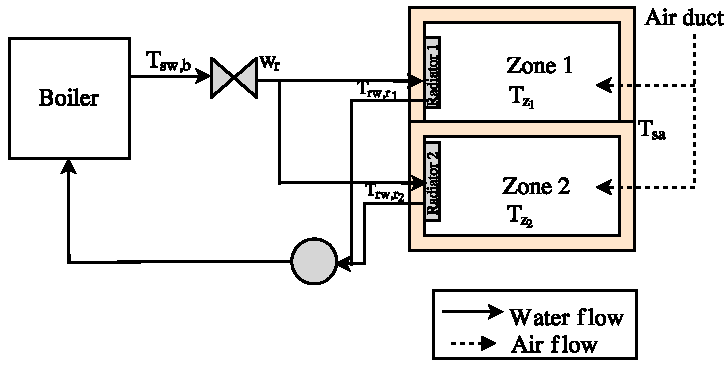
\includegraphics[width=0.5\columnwidth]{figures/Cs1.pdf}
 	\caption{figure}{BAS setup for the first case study}
 	\label{fig:cs1:setup}
 \end{figure}
 
We consider two zones, each heated by one radiator and with a common supply air, as portrayed in Figure~\ref{fig:cs1:setup}. 
The model is described as stochastic linear discrete-time model
\begin{equation}\label{mod:s}
	\textbf{M}_s: \begin{cases}
	x[k+1] &=Ax[k] + Bu[k] + Q + \Sigma W[k] \\ % \in \Rl^4 \\
	y_s[k] &= \begin{bmatrix}
	1&0&0&0\\
	0&1&0&0\end{bmatrix} x[k], 
	\end{cases}
\end{equation}
with a uniform sampling time $\Delta=$ 15 minutes. Here, the matrices $A, \; B, \; Q $ are properly sized  and \resizebox{0.55\textwidth}{!}{$ \Sigma = diag([(\sqrt{\Delta}\sigma_{z_1})^2 \; (\sqrt{\Delta}\sigma_{z_2})^2 \;(\sqrt{\Delta}\sigma_{rw,r_1})^2 \;(\sqrt{\Delta}\sigma_{rw,r_2})^2])$}
encompasses the variances of the process noise for each state. $W = \begin{bmatrix}w_1& w_2& w_3& w_4\end{bmatrix}^T$ are independent Gaussian random variables, which are also independent of the initial condition of the process. The exact matrix values are kept within the ARCH repository.

\subsubsection{CS1BAS: Specifications}
We consider the stochastic safety property:  to decide whether traces generated by the models remain within a specified safe set for a given time period. Specifically, this is described using the PCTL property:
\begin{equation*}
\Phi:= \mathbb{P}_{= p} [\square^{\le N=1.5\text{hours}}\; \mathcal{S}]
\end{equation*}
where $p$ is the probability of satisfaction, $\mathcal{S}$ is the safe set is described as an interval around the temperature set-point $T_{SP} = 20^oC$ $\pm 0.5^oC$, specifically, 
\begin{align*}
\mathcal{S}&=\begin{bmatrix}
19.5 & 20.5 \\
19.5 & 20.5 \\
19.5 & 20.5 \\
19.5 & 20.5 \\
\end{bmatrix}.
\end{align*}
We defined the acceptable probability of the specification to be true for $p \ge 0.9$.

\subsubsection{CS2BAS: Model} 
In this second case study we focus on the {stochastic} dynamics of the zone component. The model is a discrete-time model with a sampling time $\Delta = 15$ minutes, and takes the form of
\begin{equation}
	\textbf{M}_{c}:
	\begin{cases}
	x_c[k+1] &= 
	A_{c}x_c[k] +B_cu_c[k]	+ F_{c}d_c[k]+ Q_c\\
	y_c[k]   &= \begin{bmatrix}
	1&0&0&0&0&0&0 \end{bmatrix}x_c[k]. 
	\end{cases}%$}
	\label{eqn:Mc}
\end{equation}
Here the continuous state variable $x_c$ is composed of 7 states representing the zone and wall temperatures, the input $u_c$ corresponds of the fan supply rate having a dimension of 1. The disturbance vector $d_c$ has a dimension of 6 which represent external heat sources (weather, occupancy, radiators), while $Q_c$ represents constant additive terms within the model. We model the disturbances as random external effects following  Gaussian distributions with a mean $\mu$ and variance $\sigma$,  affecting the room temperature dynamics as $T_{out}[k] \sim  \mathcal{N}(\mu=9,\sigma=1),~T_{hall}[k] \sim \mathcal{N}(\mu=15,\sigma=1),\; CO_{2_i}[k] \sim  \mathcal{N}(\mu=500,\sigma=100), i \in \{1,2\},\;
T_{rw,r_i}[k] \sim  \mathcal{N} (\mu =35, \sigma=5), i \in \{1,2\}$.\\

\subsubsection{CS2BAS: Specifications}
We would like to synthesise a policy ensuring that the temperature within zone 1 does not deviate from the set point by more then 0.5$^oC$ over a time horizon equal to four hours (i.e $N= 16$). This can be translated into following PCTL specification:
\begin{equation*}
\Phi:= \mathbb{P}_{= p} [\square^{\le N=16} \; |T_{z_1}-T_{SP}| \le 0.5]
\end{equation*}
over which $p$ is to be maximised for the optimal policy. Here, $T_{SP} = 20^oC$.

